\section{Modeling of cylindrically symmetric non-paraxial beams}

In the previous sections, I have shown the plane-wave expansions in multipoles for both of the approaches for comparison. In real scattering experiments, one often works with waves that are cylindrically symmetric and not plane. These are beams that are more complicated, as they can be decomposed into \textit{many} plane waves \cite{xavi}. 
This section will describe how to model a monochromatic, non-paraxial, and cylindrically symmetric beam with a well-defined helicity using the \textit{aplanatic lens model}, which is explained both in \cite{nanooptics} and \cite{xavi}. Then, a brief description of the implementation will be given along with different visualisations of the fields.

\subsection{The aplanatic lens model}
The idea of the aplanatic lens model is to describe a focused beam as a transformation by a lens of an incident beam. In later chapters, a scattering sphere will be placed in the focal point of this lens, \( f \), making the model quite realistic. The focusing is illustrated below.

\begin{figure}
    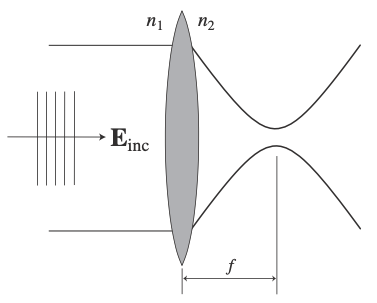
\includegraphics[width=0.5\linewidth]{Figures/aplanatic_lens.png}
    \caption{Sketch of the focusing of a light beam (here represented only by its electric field) by an aplanatic lens \cite{nanooptics}.}
    \label{fig:aplanatic}
\end{figure}

I will not go through the derivation of the expression for the focused field in great detail, but only lay out the overall steps.

The model assumes the so-called sine condition, which states that the refraction by the aplanatic lens is equivalent to that of a perfect sphere with radius \( f \). Additionally, conservation of intensity is assumed during refraction. \( \mathbf{E}_{inc} \) is then transformed from cylindrical coordinates into spherical after the lens. Some simplifications are made to ensure the conservation of helicity \( p \) and angular momentum \( J_z \). This is important, as one can then define an incident field and be certain that its important parameters are still conserved after focusing (helicity \( p = 1 \) will be used in this study).

The focused field, which naturally depends on the expression of the incident field, can be expressed as an expansion in multipoles. In \cite{xavi}, the multipolar decomposition of a Laguerre-Gaussian beam is provided. The modes of such a beam, \( \mathrm{LG}_l^q \), are cylindrically symmetric solutions of the paraxial equation. \( q \), the so-called radial index, is assumed to be 0 throughout this report, while \( l \in \mathbb{Z} \), which is related to the AM content, will be varied.

When focused by an aplanatic lens, an electric field containing LG modes becomes a solution of not only the paraxial equation but also Maxwell's equations \cite{xavi}. Such a field with a single LG mode has the expression:
\begin{equation}\label{eq:Efoc}
    \mathbf{E}_{foc} = \sum_{j=\lvert m_z \rvert}^\infty i^j \sqrt{2j+1} C_{jm_z p} \left[ \mathbf{A}_{jm_z}^{(m)} + i p \mathbf{A}_{jm_z}^{(e)} \right]
\end{equation}
where \( m_z = l + p \). The linear combination of the multipoles in the brackets is a multipole with a well-defined helicity, which will be used later. Note that the lowest multipolar order is \( \lvert m_z \rvert \).

\( C_{jm_z p} \), the coefficient whose absolute value squared describes the content of each multipole in the expansion, is given by the following expression:
\begin{align}
    \label{eq:C_foc}
    C_{jm_z p} &= \frac{f \mathrm{e}^{-i k f}}{2 \pi} \sqrt{\frac{n_1}{n_2}} \cdot \\
    &\int_0^{\theta_k^{m}} \mathrm{d} \theta_k \sin \theta_k \sqrt{\cos \theta_k} d^j_{m_z p}(\theta_k) N_l^q \mathrm{exp} \left[ -\frac{(f \sin \theta_k)^2}{w^2} \right] (f \sin \theta_k)^l L_q^l \left( \frac{2 (f \sin \theta_k)^2}{w^2} \right) \left( \frac{\sqrt{2}}{w} \right)^{l+1}
\end{align}
The integral is carried out over \( \theta_k \), a momentum-space representation of \( \theta \). This range is defined by the numerical aperture (NA) of the lens. 
Everything from \( N_l^q \) and after is the expression of the \( \mathrm{LG} \)-mode with a waist \( w \), also including a generalized Laguerre polynomial. \( N_l^q \) is a normalisation factor, and \( d^j_{m_z p}(\theta_k) \) is the reduced Wigner rotation matrix - a neat transformation that ensures that the scalar wave functions are always eigenstates of \( \mathbf{J}^2 \) and \( J_z \).

\subsection{Implementation and visualisation}
Using the multipoles as expressed in the previous chapter, focused fields can be plotted in 3D.

\begin{figure}
    \begin{subfigure}[b]{0.49\textwidth}
        \centering
        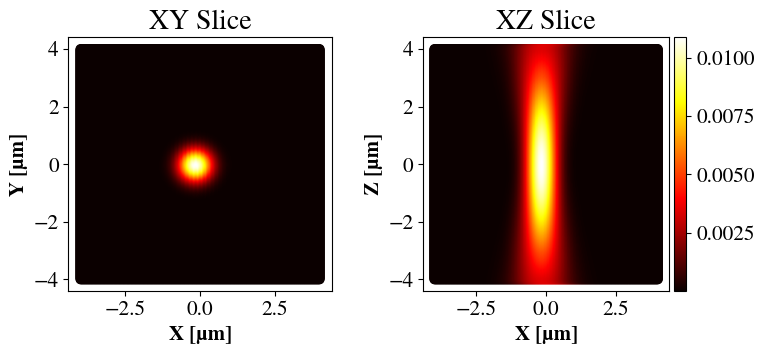
\includegraphics[width=\textwidth]{Figures/Efoc_NA5_l0.png}
        \caption{NA=0.5, \( l=0 \), \( w=270\ \mathrm{\upmu m} \)}
        \label{fig:a}
    \end{subfigure}
    \begin{subfigure}[b]{0.49\textwidth}
        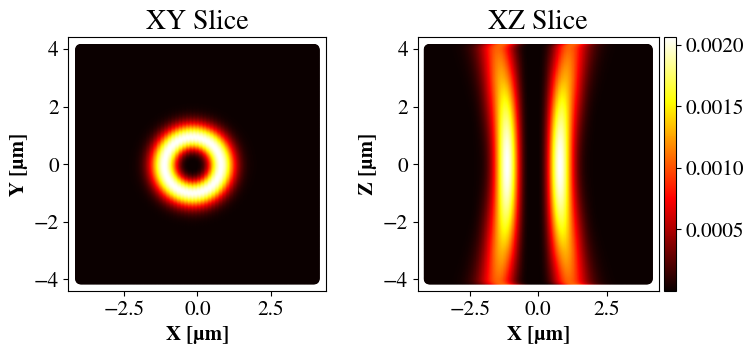
\includegraphics[width=\textwidth]{Figures/Efoc_NA5_l2.png}
        \caption{NA=0.5, \( l=2 \), \( w=216\ \mathrm{\upmu m} \)}
        \label{fig:b}
    \end{subfigure}

    \par

    \begin{subfigure}[b]{0.49\textwidth}
        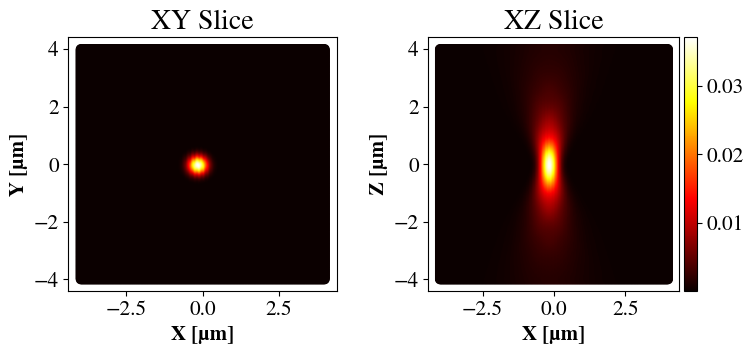
\includegraphics[width=\textwidth]{Figures/Efoc_NA9_l0.png}
        \caption{NA=0.9, \( l=0 \), \( w=500\ \mathrm{\upmu m} \)}
        \label{fig:c}
    \end{subfigure}
    \begin{subfigure}[b]{0.49\textwidth}
        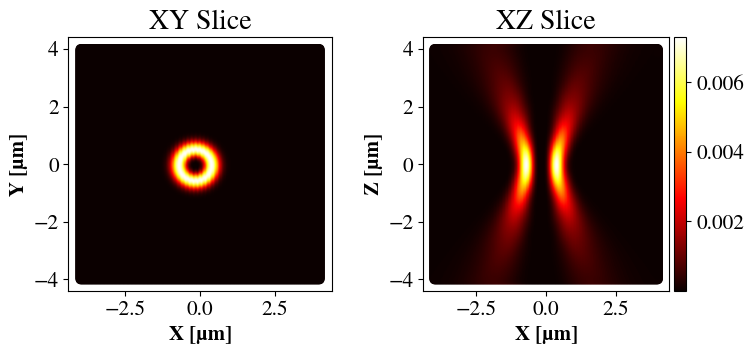
\includegraphics[width=\textwidth]{Figures/Efoc_NA9_l2.png}
        \caption{NA=0.9, \( l=2 \), \( w=390\ \mathrm{\upmu m} \)}
        \label{fig:d}
    \end{subfigure}

    \caption{2D slices of 3-dimensional intensity plots of focused z-propagating LG beams for different lens and beam parameters. XY slices correspond to a transverse slice of the beam. The XZ slices show the beam along its direction of propagation.}
    \label{fig:Efoc}
\end{figure}

Examples of focused beams are shown in the following figure for two values of NA. Clearly, higher NA gives a tighter focus, judging by the spot sizes for the \( l=0 \) cases and the curvatures for \( l=2 \). 
An interesting feature is that when \( l=0 \), the LG beam corresponds to a Gaussian beam, having highest intensity in the center. For \( l > 0 \), the beam is toroidal with no intensity in the center. 
An important point is that one can in principle vary the beam waist independently of the NA and \( l \). However, since \( l \) affects the beam shape and the NA essentially dictates the size of the lens, I have chosen \( w \) such that the beam always spans the entire lens but never exceeds it (which would mean that the beam was cut off).

Another interesting study is the multipolar content of the beams, i.e., the modal distribution in the expansions. This will be important later on, since the multipolar content directly impacts the modes excited during scattering.

For NA=0.5 and 0.9, the multipolar content, \( \lvert C_{jm_z p} \rvert^2 \), is plotted for incident beams with values \( l=0, 2, 4 \), and 6 in the histograms. Note that there are no multipoles of order \( j < l + p \). 
It is clearly seen that the more tightly focused light (NA=0.9) contains fewer, lower-ordered multipoles. As \( l \) increases, both distributions shift to higher order and become broader. A tendency toward a symmetric bell-curve is seen, especially for NA=0.5.

\begin{figure}
    \begin{subfigure}[b]{0.49\textwidth}
        \centering
        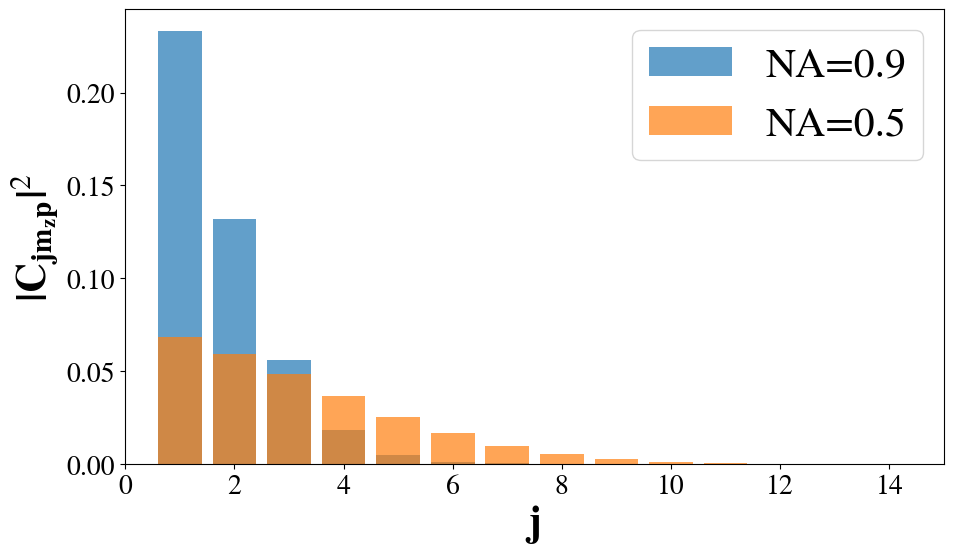
\includegraphics[width=\textwidth]{Figures/contentl0.png}
        \caption{\( l=0 \)}
        \label{fig:aa}
    \end{subfigure}
    \begin{subfigure}[b]{0.49\textwidth}
        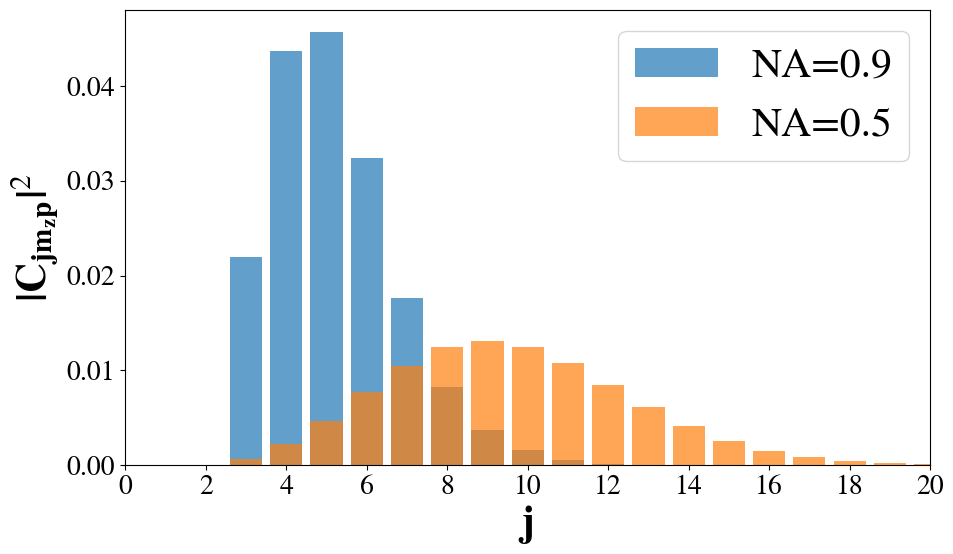
\includegraphics[width=\textwidth]{Figures/contentl2.png}
        \caption{\( l=2 \)}
        \label{fig:bb}
    \end{subfigure}

    \par

    \begin{subfigure}[b]{0.49\textwidth}
        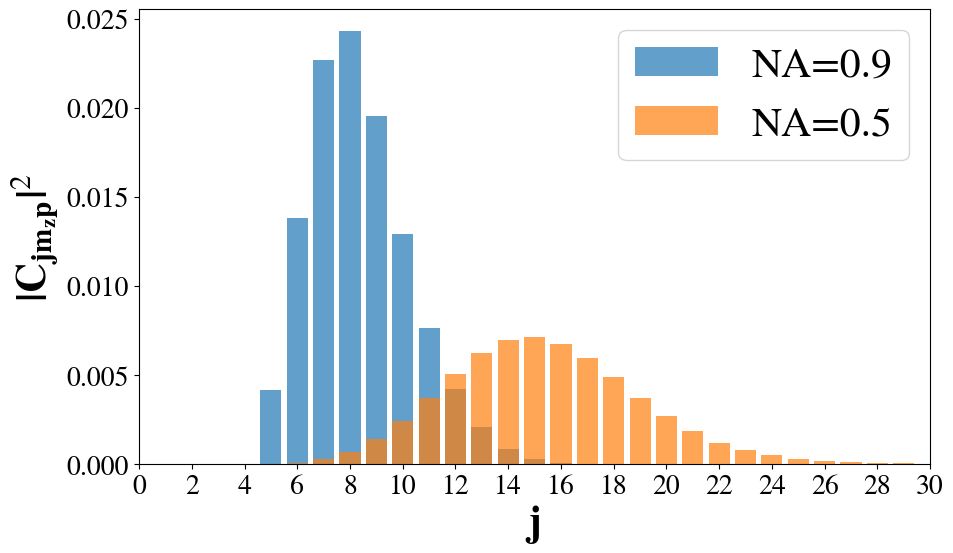
\includegraphics[width=\textwidth]{Figures/contentl4.png}
        \caption{\( l=4 \)}
        \label{fig:cc}
    \end{subfigure}
    \begin{subfigure}[b]{0.49\textwidth}
        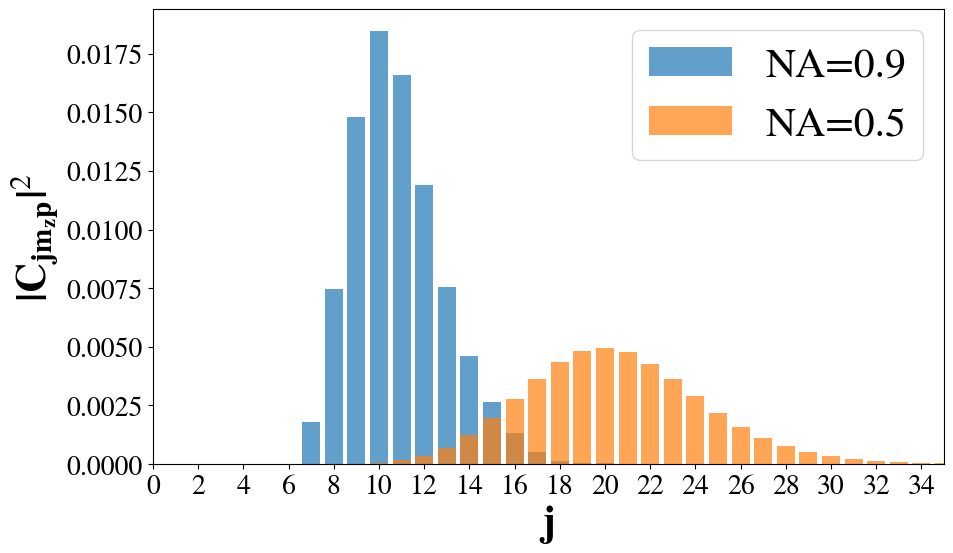
\includegraphics[width=\textwidth]{Figures/contentl6.png}
        \caption{\( l=6 \)}
        \label{fig:dd}
    \end{subfigure}

    \caption{Histograms of the multipolar content of the expansion for the focused beam. \( \lvert C_{jm_z p} \rvert^2 \) is plotted for each order \( j \) for NA=0.9 (blue) and NA=0.5 (orange) for four values of the quantum number, \( l \).}
    \label{fig:mcontent}
\end{figure}

In fact, for NA=0.9, the multipolar distribution is shown for \( l=0 \) to \( l=8 \) in the figure below to the left, showing the same trend as the histograms: that the distribution broadens and shifts toward higher \( j \).

\begin{figure}
    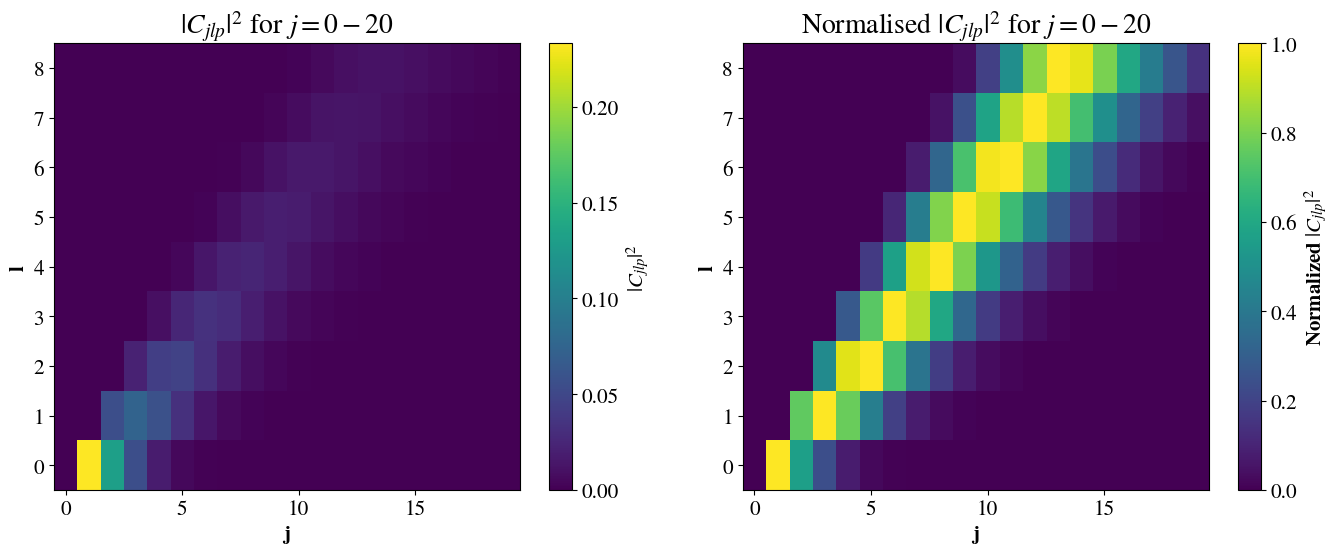
\includegraphics[width=0.9\linewidth]{Figures/C_NA09.png}
    \caption{Colour plot of the multipolar distribution of \( \lvert C_{jm_z} \rvert^2 \) for \( l=0 \) to \( l=8 \) for NA=0.9. The values on the left are on absolute scale. On the right, each row (\( l \)) is normalised to its own maximum, highlighting the dominant modes more.}
    \label{fig:Cj_NA09}
\end{figure}